\documentclass{article} % For LaTeX2e
\usepackage{amsmath, amsfonts, amsthm, amssymb}
\usepackage{nips14submit_e,times}
\usepackage{hyperref}
\usepackage{url}
\usepackage{graphicx}
\usepackage{mathrsfs}

% For bibliography
\usepackage[round]{natbib}
\renewcommand{\bibsection}{}

\title{Information Theoretic Estimators for Dependence in Time Series}

\author{
Shashank Singh \\
Statistics \& Machine Learning Departments \\
Carnegie Mellon University \\
Pittsburgh, PA 15213 \\
\texttt{sss1@andrew.cmu.edu}
}

\newcommand{\fix}{\marginpar{FIX}}
\newcommand{\new}{\marginpar{NEW}}

%%%%%%%%%%%%%%%%%%%%CONTENT MACROS%%%%%%%%%%%%%%%%%%%%%%%%%
\renewcommand{\qed}{\quad \ensuremath{\blacksquare}}    % QED blacksquare
\newcommand{\inv}{^{-1}}                            % inverse operator
\newcommand{\sminus}{\backslash}                    % set minus
\newcommand{\N}{\mathbb{N}}                         % natural numbers
\newcommand{\R}{\mathbb{R}}                         % real numbers
\newcommand{\pow}{\mathcal{P}}                      % power set
\newcommand{\Se}{\mathcal{S}}                       % partition
\newcommand{\e}{\varepsilon}                        % \varepsilon
\newcommand{\X}{\mathcal{X}}                        % X domain
\newcommand{\Y}{\mathcal{Y}}                        % Y domain
\newcommand{\Z}{\mathcal{Z}}                        % Z domain
\newcommand{\A}{\mathcal{A}}                        % sub-domain
\newcommand{\E}{\mathbb{E}}                         % expected value
\newcommand{\V}{\mathbb{V}}                         % variance
\newcommand{\pr}{\mathbb{P}}                        % probability
\newcommand{\vi}{{\vec{i}}}                         % multi-index vector i
\newcommand{\dist}{\operatorname{dist}}             % distance operator
\newcommand{\acro}[1]{\textsc{\MakeLowercase{#1}}}
\renewcommand{\hat}{\widehat}
\renewcommand{\tilde}{\widetilde}
%%%%%%%%%%%%%%%%%%%%%%%%%%%%%%%%%%%%%%%%%%%%%%%%%%%%%%%%%%%

\newcommand\ind{\protect\mathpalette{\protect\independenT}{\perp}}
\def\independenT#1#2{\mathrel{\rlap{$#1#2$}\mkern2mu{#1#2}}}

% \nipsfinalcopy % Uncomment for camera-ready version

\begin{document}

\maketitle

\begin{abstract}
Recently, there has been much interest in designing and analyzing estimators
for information theoretic functionals of probability density functions, under
the assumption of independent and identically distributed (IID) data. However,
estimators designed for IID data fail to capture relevant information when
presented with time series data. We first present information theoretic
functionals which take into account temporal dependence patterns, and then
discuss methods for estimating these functionals. We then present an empirical
evaluation of these estimators, in which we study the abilities of different
estimators to detect dependencies in different types of synthetic data. This
reveals novel patterns in the performance of these estimators over varying
inputs, resulting in new understanding of the regimes in which different
methods should be used to measure dependence between variables.
\end{abstract}

\section{Introduction}
Information theoretic functionals of probability density functions, including
entropy, mutual information, divergence, and their conditional variants, are
important nonparametric measures of variation, dependence, and distance between
random variables. Over the past few years, much work as gone into designing and
characterizing estimators for such functionals, using independent and
identically distributed (IID) samples from each of the relevant variables.

However, many data sources, such as neurophysiological, economic, and
meteorological data, consist of time series, where samples of each variable are
not independent. When analyzing such data, it may often be useful to perform
analyses using estimators for information theoretic functionals that were
designed for IID data.

One particularly common use for information theoretic functionals is to
estimate the strength of dependence between variables. If we simply
treat two time series signals as sequences of IID samples and estimate the
mutual information between them using previous methods, we are likely to fail
to capture dependencies that manifest over multiple time steps.
For example, to study functional connectivity in fMRI data, one might try to
learn a graphical model over activity in different brain regions via the
Chow-Liu or PC algorithm, which can use estimates of (conditional) mutual
information as subroutines. If, in response to a stimulus, one brain region
consistently activates a few seconds a second brain region, these brain regions
ought to be considered as functionally connected, by typical information
theoretic measures will fail to capture this dependence.

Thus, the broad goal of this work is to understand how methods using these
functionals and their estimators can be adapted for time series data.
In this paper, we focus on information theoretic functionals used to measure
dependence, although some ideas of our work extend naturally to other
functionals of interest. In particular, the two functionals we study in detail
are transfer entropy and the mutual information rate, discussed in Sections
\ref{sec:TE} and \ref{sec:MIR}, respectively.

\section{Problem Setup and Notation}
Suppose we observe two finite time series $\X = \{X_i\}_{i = 1}^n$ and
$\Y = \{Y_i\}_{i = 1}^n$ (which can be written as a joint time series
$(\X, \Y) = \{(X_i,Y_i)\}_{i = 1}^n$). We assume that the observations come
from a stationary time series (i.e., that their joint densities are invariant
to time shifts). In general, the $2n$ variables in $\{(X_i,Y_i)\}_{i = 1}^n$
can have any dependence structure. However, in order to estimate quantities of
interest, we will have to assume some independence in the form of Markov or
mixing assumptions. For $\beta \geq 1$, a $\beta$-Markov assumption holds if,
for each $i \in \{\beta + 1,\dots,n\}$,
\begin{equation}
(X,Y)_i \ind \{(X_j,Y_j)\}_{j = 1}^{i - (\beta + 1)}
                                    | \{(X_j,Y_j)\}_{j = i - \beta}^{i - 1},
\label{joint_markov}
\end{equation}
\begin{equation}
(X,Y)_i \ind \{X_j\}_{j = 1}^{i - (\beta + 1)}
                                            | \{X_j\}_{j = i - \beta}^{i - 1}
    \quad \mbox{ and } \quad
(X,Y)_i \ind \{Y_i\}_{j = 1}^{i - (\beta + 1)}
                                        | \{Y_j\}_{j = i - \beta}^{i - 1}.
\label{marginal_markov}
\end{equation}
Mixing assumptions come in several forms and are generally more complicated,
both to define and to verify for real data. Thus, we discuss them only where
necessary in our theoretical work in the Supplementary Material, where they
determine the rate of convergence of ours estimators.

\section{Related Work}
\citet{amblard2012relation} review the histories of and theoretical
relationships between direction information, Granger causality, and the mutual
information rate. However, they do not give empirical evaluation of the these
quantities, and do not discuss estimation of the relevant information theoretic
quantities. Otherwise, there has been much recent work on estimating
information theoretic functionals in the case of IID data
\citep{pal2010estimation,nguyen2010estimating,singh14densityfunc,krishnamurthy14divergences,moon14ensemble,gao2014stronglyDependent}.

% TODO: See Hlavackova-Schindler et al (2007) \emph{Causality detection based
% on information-theoretic approaches in time series analysis}. Phys. Rep.

\section{Transfer Entropy}
\label{sec:TE}
One information theoretic functional that has been studied previously is the
notion of transfer entropy (actually a case of conditional mutual information),
defined for general time series $\X$ and $\Y$ as
\[T_{\X \to \Y}^n
    = H(Y_n | \{Y_i\}_{i = 1}^{n - 1}) - H(Y_n | \{X_i\}_{i = 1}^{n - 1}, \{Y_i\}_{i = 1}^{n - 1})
    = I(Y_n; \{X_i\}_{i = 1}^{n - 1} | \{Y_i\}_{i = 1}^{n - 1}).
\]
Thus, transfer entropy can be equivalently thought of as the reduction in
uncertainty of $Y_n$ upon learning $\{X_i\}_{i = 1}^n$ when one already knows
$\{Y_i\}_{i = 1}^n$, or the mutual information between the last point of $Y$
and the previous values of $X$ given the previous values of $Y$. Thus, it
roughly measures the predictive power of $X$ on $Y$ after accounting for
autocorrelation and can be used in this sense as a dependence measure among
time series.

\subsection{Estimating Transfer Entropy}
The transfer entropy $T_{\X \to \Y}^n$ of $\{X_1\}_{i = 1}^n$ on
$\{Y_1\}_{i = 1}^n$ is a mutual information between the $1$-dimensional
variable $Y_n$ and the $(n - 1)$-dimensional variable $X_{1:(n - 1)}$
conditioned on the $(n - 1)$-dimensional variable $Y_{1:(n - 1)}$ (a $2n - 1$
dimensional conditional mutual information). Without making parametric or
independence assumptions, this makes estimating transfer entropy, very
difficult for all but very small $n$ (even when given several samples of the
entire time series). To make estimation more tractable, we reduce the dimension
of the problem by making a $\beta$-Markov assumption.
Transfer entropy then reduces to
\begin{align*}
T_{\X \to \Y}^n
 &  = H(Y_n | \{Y_i\}_{i = 1}^{n - 1})
        - H(Y_n | \{X_i\}_{i = 1}^{n - 1}, \{Y_i\}_{i = 1}^{n - 1}) \\
 &  = H(Y_n | \{Y_i\}_{i = n - \beta}^{n - 1})
        - H(Y_n | \{X_i\}_{j = i - \beta}^{i - 1}, \{Y_i\}_{j = i - \beta}^{i - 1}) \\
 &  = I(Y_n; \{X_i\}_{i = i - \beta}^{n - 1}
                                            | \{Y_i\}_{i = i - \beta}^{n - 1}).
\end{align*}
which now involves at most $\beta$-dimensional variables (a $2\beta + 1$
dimensional conditional mutual information). When $\beta \ll n$, this makes
estimation tractable. In particular, estimating transfer entropy reduces to
estimating a low-dimensional conditional entropy. This conditional entropy was
then estimated using previously derived methods, as discussed in the
Supplementary Material.

% TODO: \section{Directed Information}
% The directed information $I_{\X \to \Y}$ is defined by
% \begin{align*}
% I_{\X \to \Y}
%  &  = H(\Y) - \sum_{i = 1}^n
%                     H(Y_i | \{Y_j\}_{j = 1}^{i - 1}, \{X_j\}_{j = 1}^i) \\
%  &  = \sum_{i = 1}^n H(Y_i | \{Y_j\}_{j = 1}^{i - 1})
%                     - H(Y_i | \{Y_j\}_{j = 1}^{i - 1}, \{X_j\}_{j = 1}^i)
%     = \sum_{i = 1}^n T_{\X \to \Y}^i.
% \end{align*}
% Thus, directed information measures the total transfer entropy over the course
% of the time series. Probably, when estimating the quantities for stationary,
% $\beta$-Markov time series, this isn't very different (up to scaling by $n$)
% from transfer entropy.

\section{Mutual Information Rate}
\label{sec:MIR}
Yet another information theoretic measure of dependence between two time series
is the mutual information rate (MIR), defined for a joint time series
$(\X,\Y) = \{(X_i,Y_i)\}_{i = 1}^\infty$ by
\[I_R(\X,\Y)= \lim_{n \to \infty} \frac{I(X_1,\dots,X_n;Y_1,\dots,Y_n)}{n},\]
when this limit exists. Like transfer entropy, high dimensionality makes
estimation difficult, except for short time series of many samples, and so, to
make estimation tractable, we will assume $\beta$-Markov conditions
(\ref{joint_markov}) and (\ref{marginal_markov}) as above. We first discuss
some results for the simpler case of estimating the entropy rate of a single
time series, and then build up to estimating the MIR.

\subsection{Estimating the Entropy Rate}
Under $\beta$-Markov assumptions, then entropy rate $H_R(\X)$ reduces to
\begin{equation}
H_R(\X)
    = \lim_{n \to \infty} H(X_n | \{X_i\}_{i = 1}^{n - 1})
    = \lim_{n \to \infty} H(X_n | \{X_i\}_{i = n - \beta}^{n - 1}).
\label{eq:reduced_HR}
\end{equation}
Thus, if we can estimate the conditional distribution of
$X_n | \{X_i\}_{i = n - \beta}^{n - 1}$, then we can attempt to use a plugin
estimator. For an ergodic Markov chain with finite state space $S$ (e.g., if
$\beta = 1$
\footnote{The condition $\beta = 1$ is not restrictive here, because any
ergodic $\beta$-order Markov chain is equivalent to an ergodic first-order
Markov chain with $\beta$-dimensional states. $\beta$ continues to play a
significant role in the convergence rates of the estimators, however.}
and the conditional distribution
$\pr\left[ X_{i + 1} = x_\ell \middle| X_i = x_j \right]$ is bounded below),
the usual maximum likelihood estimate
\footnote{For any event $A$, $1_A$ denotes the indicator function of $A$.}
\[\hat \pi_{x,\{y_i\}_{i = 1}^\beta}
    =   \frac{\sum_{i = \beta + 1}^n 1_{\{X_i = x,
            \{X_i\}_{i = n - \beta}^{n - 1} = \{y_i\}_{i = 1}^{\beta}\}}}
        {\sum_{i = \beta + 1}^n
        1_{\{\{X_i\}_{i = n - \beta}^{n - 1} = \{y_i\}_{i = 1}^{\beta}\}}}
\]
of $\pr\left[ X_n = x
    \middle| \{X_i\}_{i = n - \beta}^{n - 1} = \{y_i\}_{i = 1}^{\beta} \right]$
(for each combination $x,y_1,\dots,y_\beta \in S$) used for IID data is
consistent (and, in fact, asymptotically normal). \cite{ciuperca05entropyRate}
show that, in case of an ergodic Markov chain with finite state space, this
plug-in estimator is strongly consistent and asymptotically normal as
$n \to \infty$.

\subsection{Estimating the MIR}
One might conjecture the most obvious analogue of (\ref{eq:reduced_HR}) for
MIR:
\begin{equation}
I_R(\X,\Y)
    \stackrel{?}{=}
    \lim_{n \to \infty} I(X_n; Y_n | \{(X_i,Y_i)\}_{i = n - \beta}^{n - 1}).
\label{conj:incorrect_IR}
\end{equation}
However, (\ref{conj:incorrect_IR}) does not hold due to the more complicated
effects of conditioning on mutual information (than on entropy). In particular,
we have
\begin{align}
I_R(\X;\Y)
 &  = \lim_{n \to \infty} \frac{I(X_1,\dots,X_n;Y_1,\dots,Y_n)}{n}          \\
 &  = \lim_{n \to \infty} \frac{H(X_1,\dots,X_n) + H(Y_1,\dots,Y_n)
                                    - H(x_1,\dots,X_n,Y_1,\dots,Y_n)}{n}    \\
\label{eq:MIR_est_form}
 &  = H_R(\X) + H_R(\Y) - H_R(\X,\Y)                                        \\
 &  = \lim_{n \to \infty} H(X_n | \{X_i\}_{i = n - \beta}^{n - 1})
                    + H(Y_n | \{Y_i\}_{i = n - \beta}^{n - 1})
                    - H(X_n,Y_n | \{(X_i,Y_i)\}_{i = n - \beta}^{n - 1})    \\
\notag
 &  = \lim_{n \to \infty} H(X_n | \{(X_i,Y_i)\}_{i = n - \beta}^{n - 1})
                        + H(Y_n | \{(X_i,Y_i)\}_{i = n - \beta}^{n - 1})
                        + T_{\Y \to \X}^n + T_{\X \to \Y}^n    \\
\label{ineq:tr_entropy}
 &      \hspace{48.5mm} - H(X_n,Y_n | \{(X_i,Y_i)\}_{i = n - \beta}^{n - 1}) \\
\notag
 &  \geq \lim_{n \to \infty} H(X_n | \{(X_i,Y_i)\}_{i = n - \beta}^{n - 1})
                    + H(Y_n | \{(X_i,Y_i)\}_{i = n - \beta}^{n - 1})    \\
\label{ineq:cond_bnd}
 &      \hspace{48.5mm} - H(X_n,Y_n | \{(X_i,Y_i)\}_{i = n - \beta}^{n - 1}) \\
 & = \lim_{n \to \infty} I(X_n; Y_n | \{(X_i,Y_i)\}_{i = n - \beta}^{n - 1})
\end{align}
where the inequality in (\ref{ineq:cond_bnd}) is due to the fact that the
transfer entropy is non-negative, with equality precisely when
$X_n \ind \{Y_i\}_{i = n - \beta}^{n - 1} | \{X_i\}_{i = n - \beta}^{n - 1}$
and
$Y_n \ind \{X_i\}_{i = n - \beta}^{n - 1} | \{Y_i\}_{i = n - \beta}^{n - 1}$
(i.e., when $T_{\Y \to \X}^n = T_{\X \to \Y}^n = 0$, or, equivalently, when information
is exchanged between $\X$ and $\Y$ only during simultaneous observations, with
not lag effect). Fortunately, we can use the estimators derived above for the
entropy rate to estimate $H_R(\X),H_R(\Y)$, and $H_R(\X,\Y)$ in
(\ref{eq:MIR_est_form}), giving the estimator
\[\hat I_R(\X,\Y) = \hat H_R(\X) + \hat H_R(\Y) - \hat H_R(\X,\Y).\]

\subsection{Information Rate and Transfer Entropy}
Notice that line (\ref{ineq:tr_entropy}) of the above included the transfer
entropies $T_{\Y \to \X}^n$ and $T_{\X \to \Y}^n$. In particular, we see that
MIR decomposes into
\[I_R(\X;\Y)
    = \lim_{n \to \infty} T_{\Y \to \X}^n + T_{\X \to \Y}^n
                    + I(X_n; Y_n | \{(X_i,Y_i)\}_{i = n - \beta}^{n - 1}).\]
Intuitively, the average information shared between $\X$ and $\Y$ can be
decomposed into the (directed) lag effects of $Y$ on $X$ ($T_{\Y \to \X}^n$),
the (directed) lag effects of $Y$ on $X$ ($T_{\X \to \Y}^n$), and the
(undirected) simultaneous shared information of $X$ and $Y$ after accounting
for history ($I(X_n; Y_n | \{(X_i,Y_i)\}_{i = n - \beta}^{n - 1})$). Contrasted
from transfer entropy, MIR is thus a coarser, more holistic (undirected)
measure of shared information between two time series. This will be further
explored empirically in Section \ref{sec:empirical}.

\section{Empirical Results}
\label{sec:empirical}
We performed experiments on synthetic data to compare the behavior of
estimators for transfer entropy, MIR, and the usual (IID) mutual information,
as well as the behaviors of two approaches to estimating these quantities,
$k$-nearest neighbor (KNN) estimators and those based on kernel density
estimates (KDE estimators).
Most previous empirical studies of information theoretic estimators
\citep{singh14densityfunc,krishnamurthy14divergences,pal2010estimation,
			  moon14ensemble,gao2014stronglyDependent}
have compared the absolute errors of estimators for distributions where the
true quantity can be computed analytically. In our experiments, we instead
compare the power of using different estimators to detect dependencies at a
fixed false positive rate. We do so for two reasons:

Firstly, we are interested in comparing the abilities of not only different
estimators, but also different information theoretic quantities to capture
dependence between variables. Transfer entropy, MIR, and mutual information
measure fundamentally different quantities, and hence the errors of their
estimators cannot be compared fairly.

Secondly, precise estimation of information theoretic functionals is (a)
unnecessary for many practical applications and (b) subject to nuanced sources
of error irrelevant to our evaluation. In most practical applications, the
estimated mutual information between two variables is itself not interpretable
or informative; rather, we are interested only how this quantity compares
across different pairs of variables, through, for example, the ranking of the
mutual information estimates over variables. Furthermore, for example,
\citet{gao2014stronglyDependent} showed that classical KNN estimators tend
severely underestimate the mutual information between variables which are
strongly dependent.
\footnote{\citet{gao2014stronglyDependent} also show that this can be corrected
by performing local dimension reduction before applying the estimators.
Intuitively, KDE estimators are also subject to this problem and can be likely
corrected using locally adaptive kernels, but this has not yet been shown.}
On the other hand, the estimated mutual information still tends, on average, to
monotonically increase with the true mutual information, and hence, given
sufficient data, we can still reliably estimate the ranking of mutual
information. As explained in the next section, out experiments rely only on the
ranking of the mutual information estimates, and are thus more robust to issues
of precise estimation such as that discussed in
\citet{gao2014stronglyDependent}. As a consequence of this robustness, we are
also able to obtain good results with in our experiments with samples that are
far smaller (by at least an order of magnitude) than previous experiments on
estimating information theoretic quantities.

\subsection{Permutation Tests for Independence}
Suppose we observe $n$ joint samples $(\X_n,\Y_n) = \{(X_i,Y_i)\}_{i = 1}^n$
from two time series $\X$ and $\Y$. Suppose also that, for some quantity
$F(\X,\Y)$, we have a consistent estimator $\hat F(\X_n,\Y_n)$ with the
property that, when $\X \ind \Y$, the distribution of $\hat F(\X_n,\Y_n)$ is
the same as the distribution of $\hat F(\X_n,\Y_{n,\sigma})$, where
$\Y_{n,\sigma} = \{Y_{\sigma(i)}\}_{i = 1}^n$ for any permutation
$\sigma : \{1,\dots,n\} \to \{1,\dots,n\}$. Under these conditions, it is easy
to see that the following procedure is a valid $\alpha$-level hypothesis test
for the null $H_0 : \X \ind \Y$:
\begin{enumerate}
\item For a large number $P$, generate $P$ permutations
$\sigma_1,\dots,\sigma_p$ uniformly at random.
\item Compute the statistic
$\hat p := \frac{1}{P} \sum_{i = 1}^P 1_{\{\hat F(X,Y) > \hat F(X,Y_\sigma)\}}$
\item Reject $H_0$ if and only if $\hat p < \alpha$.
\end{enumerate}
That is, we reject $H_0$ when $\hat F(\X_n,\Y_n)$ is greater than $1 - \alpha$
fraction of $\hat F(\X_n,\Y_{n,\sigma})$. If, additionally, $F(\X,\Y)$
satisfies $F(\X,\Y) = 0$ whenever $\X \ind \Y$ and $F(\X,\Y) > 0$ otherwise,
we expect this test to have some power against the alternative $H_1$, because
permuting $\Y$ randomly ought to break most of the dependence structure between
$\X$ and $\Y$, so that, if $\X \not\ind \Y$,
$\hat F(\X_n,\Y_{n,\sigma}) \to 0$ while $\hat F(\X_n,\Y_n) \to F(\X,\Y) > 0$.

This type of permutation test is the basis of our empirical studies in this
section, using $T_{\X \to \Y}^n$, $I$, and $I_R$ in place of $F$, and the
respective estimators discussed above in place of $\hat F$.

\subsection{Details of the Experiments}
Each experiment used $n = 300$ time samples, generated after $1000$ identical
samples that were discarded to ensure stationarity. Permutation tests used a
type I error rate of $\alpha = 0.05$ and $P = 2000$ permutations. In all of the
following experiment descriptions, $\{\e_i\}_{i \in \mathbb{Z}}$ is IID
standard Gaussian noise (i.e., each $\e_i \sim \mathcal{N}(0,1)$), and
$\{\delta_i\}_{i \in \mathbb{Z}}$ is IID zero-mean Gaussian noise with variance
$\sigma_\Y$ (i.e., each $\e_i \sim \mathcal{N}(0,\sigma_\Y)$), for each
$\sigma_\Y \in \{1,\dots,10\}$ (as seen over the $x$-axes in Figure
\ref{fig:results}). Finally, for each experiment, we tried $3$ different lags
$\beta \in \{1,2,3\}$. The same $\beta$ was used to generate the data and to
estimate the transfer entropy and mutual information rate. Note that $\beta$
does not affect on the mutual information between $X_i$ and $Y_i$ (except
indirectly through the lagged dependence in Experiment 1).

{\bf Experiment 1 (Simultaneous and Lagged Dependence):} In this experiment,
$\X$ and $\Y$ depend on each other due to both simultaneous shared noise and a
lagged direct dependence of $\Y$ on $\X$. In particular, we set
\begin{align*}
                X_{i + 1} & = \frac{X_i}{2} + \e_{i + 1}  \\
\mbox{ and }    Y_{i + 1} & = X_{i + 1 - \beta} + \e_{i + 1} + \delta_{i + 1}
\end{align*}
Because $X_{i - \beta}$ is predictive of $Y_i$ and $X_i$ shares noise $\e_i$
with $Y_i$, we expect all three of transfer entropy, mutual information, and
MIR to have some power here.

{\bf Experiment 2 (Simultaneous Dependence):} In this experiment, $\X$ and $\Y$
depend on each other only through simultaneous shared noise. In particular, we
set
\begin{align*}
                X_{i + 1} & = \frac{X_i}{2} + \e_{i + 1}  \\
\mbox{ and }    Y_{i + 1} & = \e_{i + 1} + \delta_{i + 1}
\end{align*}
Because $X_{i - \beta}$ is never predictive of $Y_i$ we expect transfer entropy
to fail here. Because $X_i$ shares noise $\e_i$ with $Y_i$, we expect mutual
information and MIR to have some power here.

{\bf Experiment 3 (Lagged Dependence):} In this experiment, $\X$ and $\Y$
depend on each other only through a lagged direct dependence of $\Y$ on $\X$.
In particular, we set
\begin{align*}
                X_{i + 1} & = \e_{i + 1}  \\
\mbox{ and }    Y_{i + 1} & = X_{i + 1 - \beta} + \delta_{i + 1}
\end{align*}
Because $X_{i - \beta}$ is never predictive of $Y_i$ we expect transfer entropy
to fail here. Because $X_i$ shares noise $\e_i$ with $Y_i$, we expect mutual
information and MIR to have some power here.

\begin{figure}[ht]
\centering
%\hspace*{-20mm}
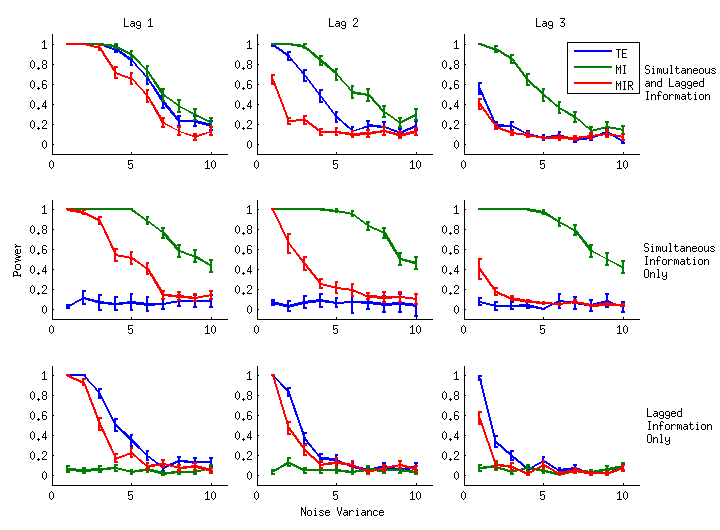
\includegraphics[width=\textwidth,clip=true,trim=3mm 3mm 0mm 0mm]{final_all}
\caption{Graphical results of our experiments. Each plot shows the power of the
permutation test for independence based on estimating each of transfer entropy,
mutual information, and MIR (higher values indicate greater power), as a
function of the noise in the dependence (i.e, the $x$-axes are roughly the
noise-to-signal ratio). Plots to the right correspond to longer range
dependencies within the time series (i.e., longer lag effects), and
correspondingly weaker independence assumptions on the time series when
computing $\hat T_{\X \to \Y}^n$ and $\hat I_R(\X,\Y)$ (i.e., increasing
$\beta$). Plots in the same row have similar dependency structure (e.g.,
simultaneous or lagged dependence). Each curve plotted is averaged over $72$
independent trials, and error bars show standard error over these trials.}
\label{fig:results}
\end{figure}

\subsection{Comparing measures of dependence}
\subsubsection{Transfer Entropy, Mutual Information, and Mutual Information
Rate Measure Different Dependence Structures}
In several respects, the estimators behaved as anticipated by design. In
Experiment 1, all three estimators were quite powerful (it is worth noting
here that the noise in all of the above simulations is at least as, if not much
more, powerful as the signal, so that demonstrating even moderate power is
fairly notable). In Experiment 2, transfer entropy failed to detect dependence,
while, in Experiment 3, mutual information failed to detect the dependence.

\subsubsection{MIR is the most general, least powerful measure}
In all three experiments, MIR detected dependence (at least for low noise),
which is consistent with the decomposition in (\ref{ineq:tr_entropy}) of MIR
into two lagged components and a simultaneous component. However, because MIR
attempts to measure multiple possible dependencies simultaneously, it uniformly
has less power than other measures which detect precisely the dependence in the
data (e.g., if there the data exhibit no lagged dependence, then the lagged
dependence terms in MIR reduce to noise, reducing the power of the permutation
test). Thus, in general, MIR should be used when there is little
\emph{a priori} reason to suspect a particular dependence structure, but a
more powerful test can be devised otherwise.

\subsection{Comparing estimators of entropy}

\subsubsection{KNN estimators scale better with dimensions}
For $\beta = 1$, across all conditions, the kernel-based entropy estimator
resulted in an average $20\%$ more power than did the KNN estimator. However,
as the lag $\beta$ increased, the performance of KDE estimators dropped
sharply, due to the strong effect of the curse of dimensionality on KDEs. On
the other hand, the performance of KNN estimators was fairly consistent as
$\beta$ increased. This phenomenon was also observed in \citet{moon14ensemble}
as the dimension of the data increases, and the performance of both KDE and KNN
approaches would likely benefit from the optimal ensemble modifications
discussed in therein.

\subsection{KDE estimators are more noise-tolerant}
On the other hand, the performance of KNN estimators degraded more quickly than
that of KDE estimators as independent Gaussian noise was added to each $Y_i$.
That is, KDE estimators appear be more tolerant to noise interfering in the
relationship between the two variables.

Notably, for small $\beta$, our estimators actually performed \emph{better} in
the presence of some noise ($\sigma = 1$) than in the noiseless case
($\sigma = 0$). This is likely a reflection of the phenomenon mentioned above
and discussed in detail in \citet{gao2014stronglyDependent}, where the mutual
information of strongly dependent variables is difficult to estimate without
using certain corrections.

\subsection{Conclusions to draw from the experiments}
The primary practical lessons to glean from the empirical results are that
\begin{enumerate}
% \item The number of permutations needed in the permutation test not be
% extremely large
\item MIR is highly reliable without prior knowledge about the dependence
structure.
\item Transfer entropy and mutual information can have higher power
if the structure of the dependence is appropriate.
\item Kernel-based estimators outperform KNN estimators in low dimensions
(small $\beta$) and can be more robust to noise, but scale poorly with $\beta$.
\item The number of samples needed to have moderate power is not particularly
large, even though quite a few samples may be needed to have small absolute
error in estimating the quantity of interest.
\item $\beta$ should be kept as small as possible, and has a significant effect
on the number of samples needed for power.
\end{enumerate}

\section{Summary and Future Work}
In this paper, we
\begin{enumerate}
\item discussed the intuition behind and relationships between some quantities
that measure dependence between time series.
\item designed estimators for these quantities.
\item empirically compared the abilities of these estimators to detect
different dependence structures under noise.
\item Compared the abilities of different estimators (KNN, KDE plug-in, etc.)
to distinguish dependent and independent time series via a permutation test.
\end{enumerate}
Additionally, in the Supplementary Material, we discuss an approach to proving
convergence of these estimators under certain mixing assumptions on the time
series.

Here, we focused primarily on estimating information theoretic functionals
which measure dependence between time series. However, estimating functionals
of probability densities from time series data can have applications to many
other problems in machine learning and data analysis. For instance, we may wish
to perform machine learning tasks over entire times series (as opposed to
individual points in time series), such as classifying entire time series as
ordinary or anomalous. Since many machine learning algorithms can operate on
distances between samples (rather than the original data points), one way to
perform such tasks is to estimate distances or divergences between the
distributions of the time series, which are often much more informative than
the original time series (see, e.g., \citet{poczos12learningOnDists}). The
convergence bounds developed in the Supplementary Material extends quite
naturally to estimating arbitrary smooth functionals of probability densities,
and so this should be developed, along with appropriate empirical evaluation.

Another potential application of these estimators is to visualizing
dependencies within high-dimensional time series data. Suppose that we jointly
measure $M$ time series, and are interested in understanding structure of these
dependencies. The pairwise dependency strengths can be computed to give an
$M \times M$ matrix, which can compared to a Gram matrix in that it represents
a sort of similarity between variables. This matrix can then be used in
combinations with standard methods such as kernel $k$-means or multidimensional
scaling (MDS), which take as input a similarity matrix.
As a concrete example, suppose we obtain measurements at each of ten weather
stations over the course of a year. In order to understand how much geographic
proximity determines the interdependence of weather phenomena across regions,
one may wish to visualize the measurements taken at different weather stations
in terms of their similarity. Our proposed method using MDS gives a way of
performing this visualization within, say, 2-dimensions, where results can be
compared to geographic coordinates after rotating and scaling.

Finally, many other tests of independence and conditional independence of
variables have been developed by others, for both time series and IID data.
These include, a mutual information based bootstrap test for independence of
time-series described in \cite{wu09bootstrapMI}, several independence tests
described in \citep{gretton10nonparametricIndependence}, and conditional
dependence measures (noting that, in principle, any conditional dependence
measure can play the role of conditional mutual information in transfer
entropy), e.g., \citep{bergsma10nonparametric} and \citep{zhang12kernel}. The
estimators and resulting permutation tests described here should be compared
empirically and theoretically to these alternatives.

\subsubsection*{References}
\setlength{\bibsep}{0.0pt}
{
%\small
\bibliographystyle{plainnat}
\bibliography{biblio}
}

\end{document}
